\documentclass[12pt]{beamer} 
% handout to collapse each frame to one page

% \renewcommand{\ttdefault}{xkcd}
% \renewcommand{\familydefault}{\ttdefault}



% compres pour afficher les "ronds" dans l'en-tete sur une seule ligne
% [compress] peut peut etre aussi se mettre dans le declaration du theme
% fleqn pour mettre un numero a droite aux equations, c'est ledno pour a droite
% cette numerotation ne marche apparement pas sous beamer...

% style beamer
%\usetheme{Darmstadt}
\usetheme{Boadilla}
%\usetheme{Warsaw}
%\usetheme{Pittsburgh }
%\usetheme{Madrid}
%\usetheme{Rochester}
%\usetheme{Copenhagen}
%\usetheme{Singapore}
%\usetheme{Malmoe}
%\usetheme{Marburg}
%\useoutertheme{miniframes}
%\useoutertheme{smoothbars}
%\usecolortheme[named=seahorse]{structure} %  utiliser avec xcolor=dvipsnames dans les options de document beamer

\usepackage[english]{babel}   % Document en anglais
\usepackage[utf8x]{inputenc}  % Accents dans le source
\usepackage{ucs}
\usepackage{amsmath}
\usepackage{amsfonts}
\usepackage{amssymb}
\usepackage{stmaryrd}
\usepackage{makeidx}
%\usepackage[svgnames]{xcolor} % Pour mettre de la couleur

\usepackage{graphicx}
\usepackage{tabularx}

\usepackage{fixltx2e}

\graphicspath{ {img/} }

\usepackage{listings}
\usepackage{caption}
\usepackage{forloop}
%\usepackage{subfig}

\usepackage{color}
%\usepackage{soul}
\usepackage[normalem]{ulem}

\definecolor{black}{rgb}{0,0,0}
\definecolor{white}{rgb}{1,1,1}
\definecolor{red}{rgb}{1,0,0}

% use xkcd font
%% Note: that's a font with no bold or italic...
\usepackage[T1]{fontenc}
%\definecolor{xkcd_color}{rgb}{.431,.482,.569}
\definecolor{xkcd_color}{rgb}{.376,.435,.533}
\usecolortheme[named=xkcd_color]{structure}
\renewcommand{\familydefault}{xkcd}
%\fontfamily{xkcd}\selectfont

%% Fallback for maths
%% http://www.tug.dk/FontCatalogue/augie/
\usepackage{emerald}
%\ECFAugie

\usepackage{textcomp} % tilde

% center titles
\setbeamertemplate{frametitle}[default][center]

% packages style
\usepackage{pslatex}
%\usepackage{graphicx}
\usepackage{multirow}
\usepackage{fancyvrb}

\usepackage[absolute,overlay]{textpos}
\newcommand{\putat}[3]{\begin{picture}(0,0)(0,0)\put(#1,#2){#3}\end{picture}}

\usepackage[autoplay]{animate}


\usepackage{listings}
\usepackage{color}
\definecolor{keywords}{RGB}{255,0,90}
\definecolor{comments}{RGB}{60,179,113}
\lstset{language=Python,
keywordstyle=\color{keywords},
commentstyle=\color{comments}\emph,
basicstyle=\scriptsize\tt}

% \renewcommand{\theFancyVerbLine}{\sffamily
% \textcolor[rgb]{0.5,0.5,1.0}{\scriptsize
% \oldstylenums{\arabic{FancyVerbLine}}}}

% from http://tex.stackexchange.com/questions/57151/how-do-i-prevent-conflicts-between-accsupp-and-hyperref
\usepackage{accsupp}
\newcommand\emptyaccsupp[1]{\BeginAccSupp{ActualText={}}#1\EndAccSupp{}}


%default definition is: \def\theFancyVerbLine{\rmfamily\tiny\arabic{FancyVerbLine}}
\let\theHFancyVerbLine\theFancyVerbLine% don't apply our patch to hyperref's version
\def\theFancyVerbLine{\rmfamily\tiny\emptyaccsupp{\arabic{FancyVerbLine}}}


% suppression de la barre de navigation
\setbeamertemplate{navigation symbols}{}

\setbeamertemplate{footline}{
\begin{beamercolorbox}[ht=2.5ex,dp=1.125ex,%
      leftskip=.3cm,rightskip=.3cm plus1fil]{}%
       \hfill    \small \insertframenumber/\inserttotalframenumber%
    \end{beamercolorbox}%
  }

% Customized title page
\defbeamertemplate*{title page}{Boadilla theme}[1][]{
  \begin{center}
    %flip image
  \scalebox{-1}[1]{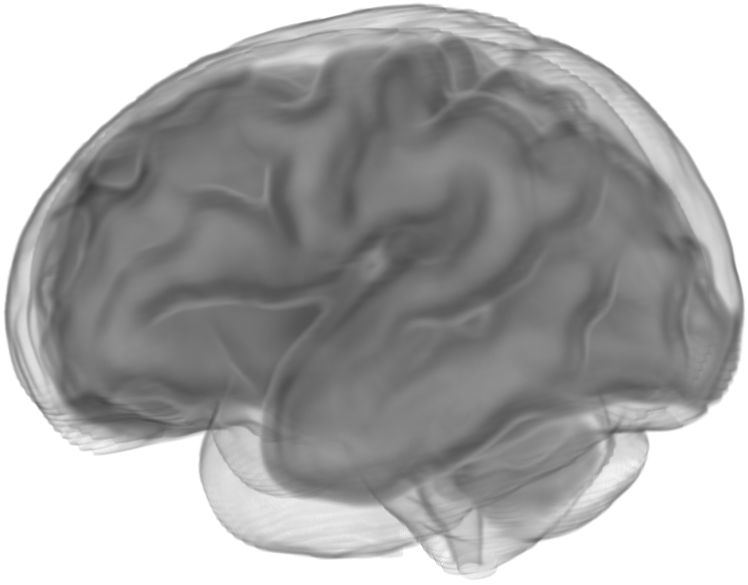
\includegraphics[width=0.4\textwidth]{brain.png}}
  \vspace{0.1\textheight}
  
  {\usebeamerfont{title}\usebeamercolor[fg]{title}\inserttitle}\par
  {\usebeamerfont{subtitle}\usebeamercolor[fg]{subtitle}\insertsubtitle}\par
  \vspace{0.05\textheight}
  {\usebeamerfont{author}\insertauthor}\par
  \vspace{0.02\textheight}
  \usebeamerfont{institute}\insertinstitute\par
  %\inserttitlegraphic\par
  \vspace{0.15\textheight}
  { \footnotesize\insertdate}\par
% \vspace{0.1\textheight}
  \end{center}
}
\title[]{Automated segmentation and motion correction of the fetal brain}
\author[K. Keraudren]{Kevin Keraudren}

\date{December 6\textsuperscript{th}, 2013}
\institute[ICL]{Imperial College London}

% image de fond
%\setbeamertemplate{background canvas}{}%{\includegraphics[width=\paperwidth,height=\paperheight]{bckgrnd.eps}}

%% \AtBeginSection[]{
%%  \begin{frame}{Outline}
%%    \small
%%    \begin{columns}
%%      \begin{column}{5cm}
%%        \tableofcontents[sections={1-4},currentsection, hideothersubsections]
%%      \end{column}
%%      \begin{column}{5cm}
%%        \tableofcontents[sections={5-8},currentsection, hideothersubsections]
%%    \end{column}
%%  \end{columns}
%% \end{frame} 
%% }
% \AtBeginSection[]{
%  \begin{frame}
%    \tableofcontents[currentsection, hideothersubsections]
% \end{frame} 
% }
\usepackage{etex}
\usepackage{tikz}
\usetikzlibrary{arrows,shapes}
%\usetikzlibrary{positioning}
\tikzstyle{na} =  [baseline=-.5ex]
\tikzstyle{nb}= [] % [baseline=10.5ex]
\usetikzlibrary{calc,decorations.pathmorphing,patterns}

% http://tex.stackexchange.com/questions/39296/simulating-hand-drawn-lines
\makeatletter
\pgfdeclaredecoration{penciline}{initial}{
    \state{initial}[width=+\pgfdecoratedinputsegmentremainingdistance,auto corner on length=1mm,]{
        \pgfpathcurveto%
        {% From
            \pgfqpoint{\pgfdecoratedinputsegmentremainingdistance}
                            {\pgfdecorationsegmentamplitude}
        }
        {%  Control 1
        \pgfmathrand
        \pgfpointadd{\pgfqpoint{\pgfdecoratedinputsegmentremainingdistance}{0pt}}
                        {\pgfqpoint{-\pgfdecorationsegmentaspect\pgfdecoratedinputsegmentremainingdistance}%
                                        {\pgfmathresult\pgfdecorationsegmentamplitude}
                        }
        }
        {%TO 
        \pgfpointadd{\pgfpointdecoratedinputsegmentlast}{\pgfpoint{1pt}{1pt}}
        }
    }
    \state{final}{}
}
\makeatother

\tikzstyle{block} = [rectangle, draw,
     text centered, minimum height=2.5em,decoration=penciline,decorate, thick]
% \tikzstyle{ellipse_block} = [ellipse, draw,
%      text centered,decoration=penciline,decorate]
\tikzstyle{line} = [draw, ->,decoration=penciline,decorate, thick]

% For every picture that defines or uses external nodes, you'll have to
% apply the 'remember picture' style. To avoid some typing, we'll apply
% the style to all pictures.
\tikzstyle{every picture}+=[remember picture]

%\setbeamertemplate{footline}[frame number]

%\everymath{\displaystyle}


\begin{document}

%\fontfamily{xkcd}\selectfont

% ------ page de titre ------
%\frame{\titlepage}[plain]
\begin{frame}[plain]
	\titlepage
\end{frame}

% ------ sommaire ------
 %[allowframebreaks]%
% \begin{frame}
% 	\tableofcontents
% \end{frame}

\begin{frame}{Problem}
\centering

As the fetuse moves

\vspace{0.02\textheight}

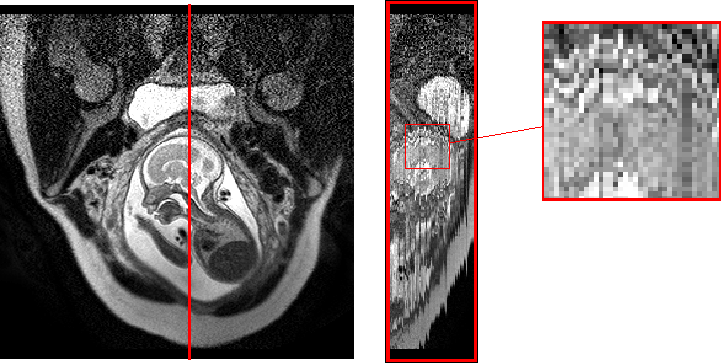
\includegraphics[width=\textwidth]{XY_plane_all.pdf}

the data is acquired as stacks of misaligned 2D slices

\end{frame}


\begin{frame}{Problem}

\centering

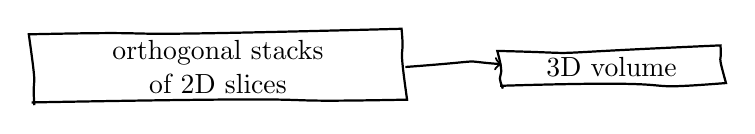
\begin{tikzpicture}[decoration=penciline]

\node[text width=4.5cm,align=center, decorate,thick,rectangle, draw] (stacks) at (0,0) {orthogonal stacks of 2D slices};

\node[text width=2.6cm,align=center, decorate,thick,rectangle, draw] (volume) at (5,0) {3D volume};

\path [draw, thick, ->, decorate]  (stacks) -- (volume);

\end{tikzpicture}


\begin{minipage}{0.45\textwidth}
\centering

    \tikz[nb]\node [] (b1)
    {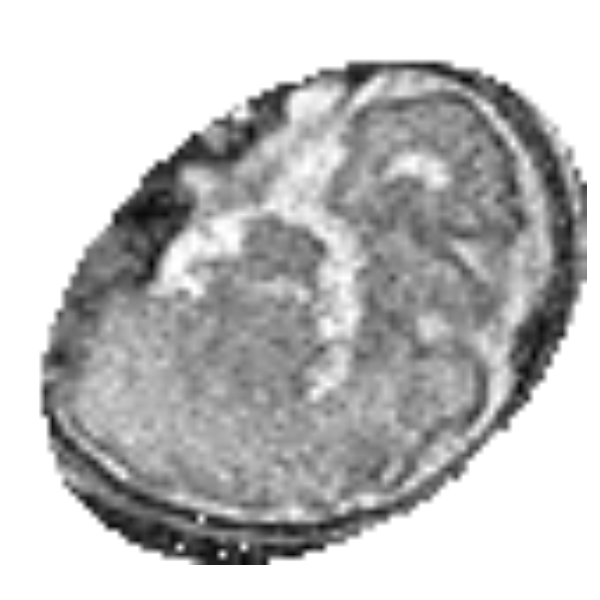
\includegraphics[angle=90,width=0.35\textwidth]{white_890_7XZ.png}
      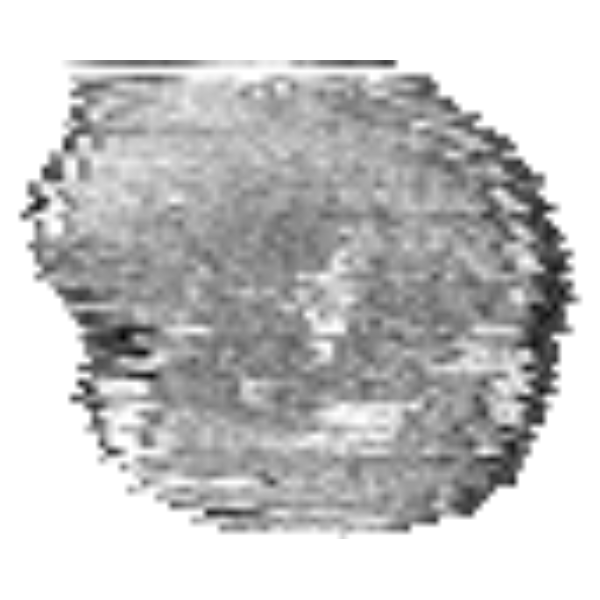
\includegraphics[width=0.35\textwidth]{white_890_7XY.png}};\\
    
    \tikz[nb]\node [] (b2)
{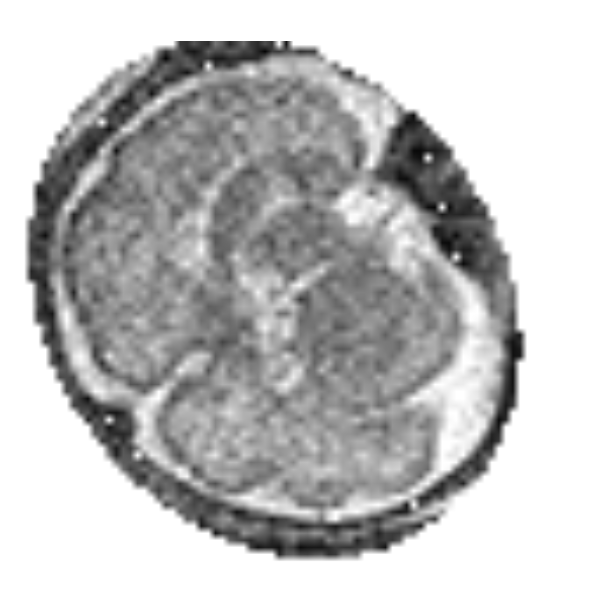
\includegraphics[angle=90,width=0.35\textwidth]{white_890_11YZ.png}
      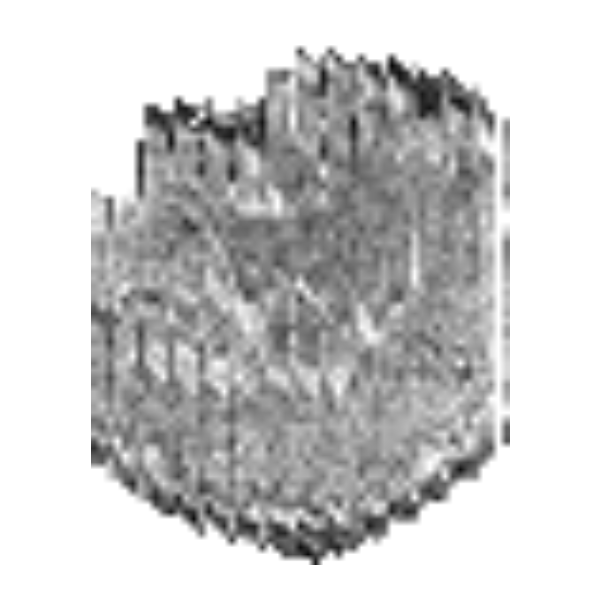
\includegraphics[width=0.35\textwidth]{white_890_11XZ.png}};\\

    \tikz[nb]\node [] (b3) 
{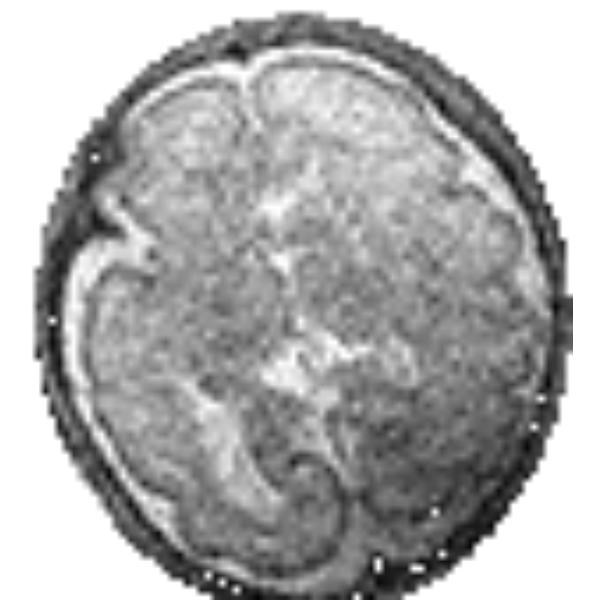
\includegraphics[width=0.35\textwidth]{white_890_1XY.png}
      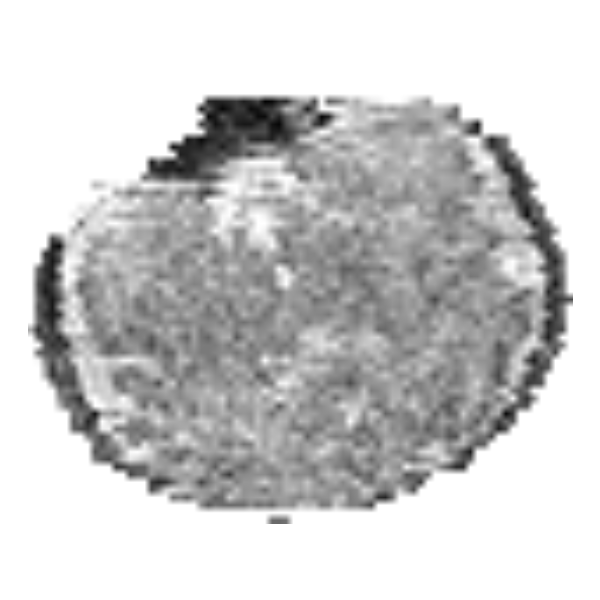
\includegraphics[width=0.35\textwidth]{white_890_1XZ.png}};\\

  \end{minipage}
\begin{minipage}{0.45\textwidth}
\centering

    \tikz[nb]\node [] (b4)
    {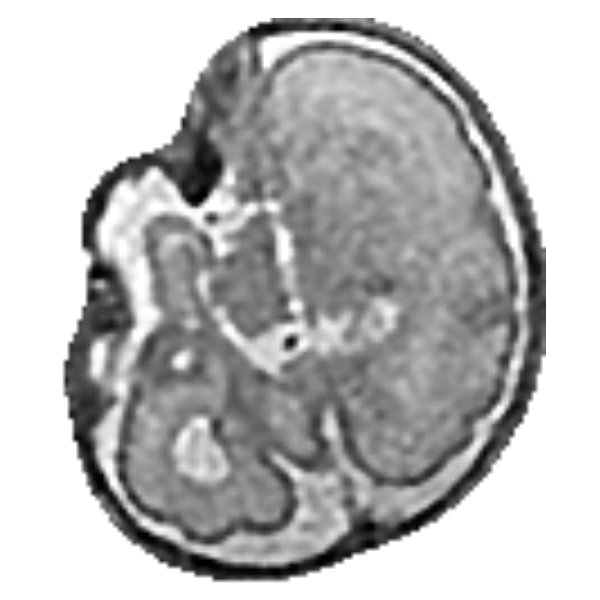
\includegraphics[angle=90,width=0.4\textwidth]{white_890_maskingXY.png}
      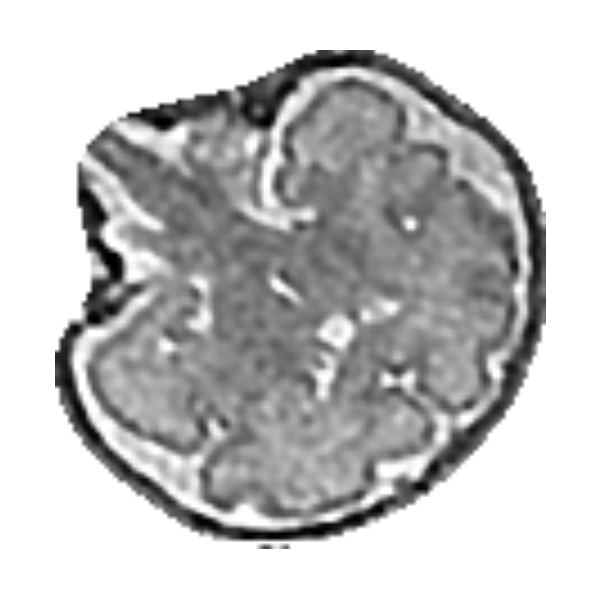
\includegraphics[angle=90,width=0.4\textwidth]{white_890_maskingXZ.png}};
      
\end{minipage}

  \begin{tikzpicture}[overlay,decoration=penciline]
    \path[black,thick,rounded corners] (b1) edge[decorate,out=-15, in=180] (b4);
    \path[black, thick,rounded corners] (b2) edge[decorate,out=0, in=180] (b4);
    \path[black, thick,rounded corners] (b3) edge[decorate,out=20, in=180] (b4);   
  \end{tikzpicture}  

\end{frame}

\begin{frame}{Definitions}
\centering

\[
 \text{recall} = \frac{\text{Volume of correctly classified voxels}}
{\text{Ground truth volume of the brain}}
\]

\[
 \text{recall} = \frac{\text{TP}}{\text{TP + \textcolor{red}{FN}}}
\]

\[
 \text{precision} = \frac{\text{Volume of correctly classified voxels}}
{\text{Detected volume of the brain}}
\]

\[
 \text{precision} = \frac{\text{TP}}{\text{TP + \textcolor{red}{FP}}}
\]

\end{frame}

\begin{frame}{Idea}
\begin{center}
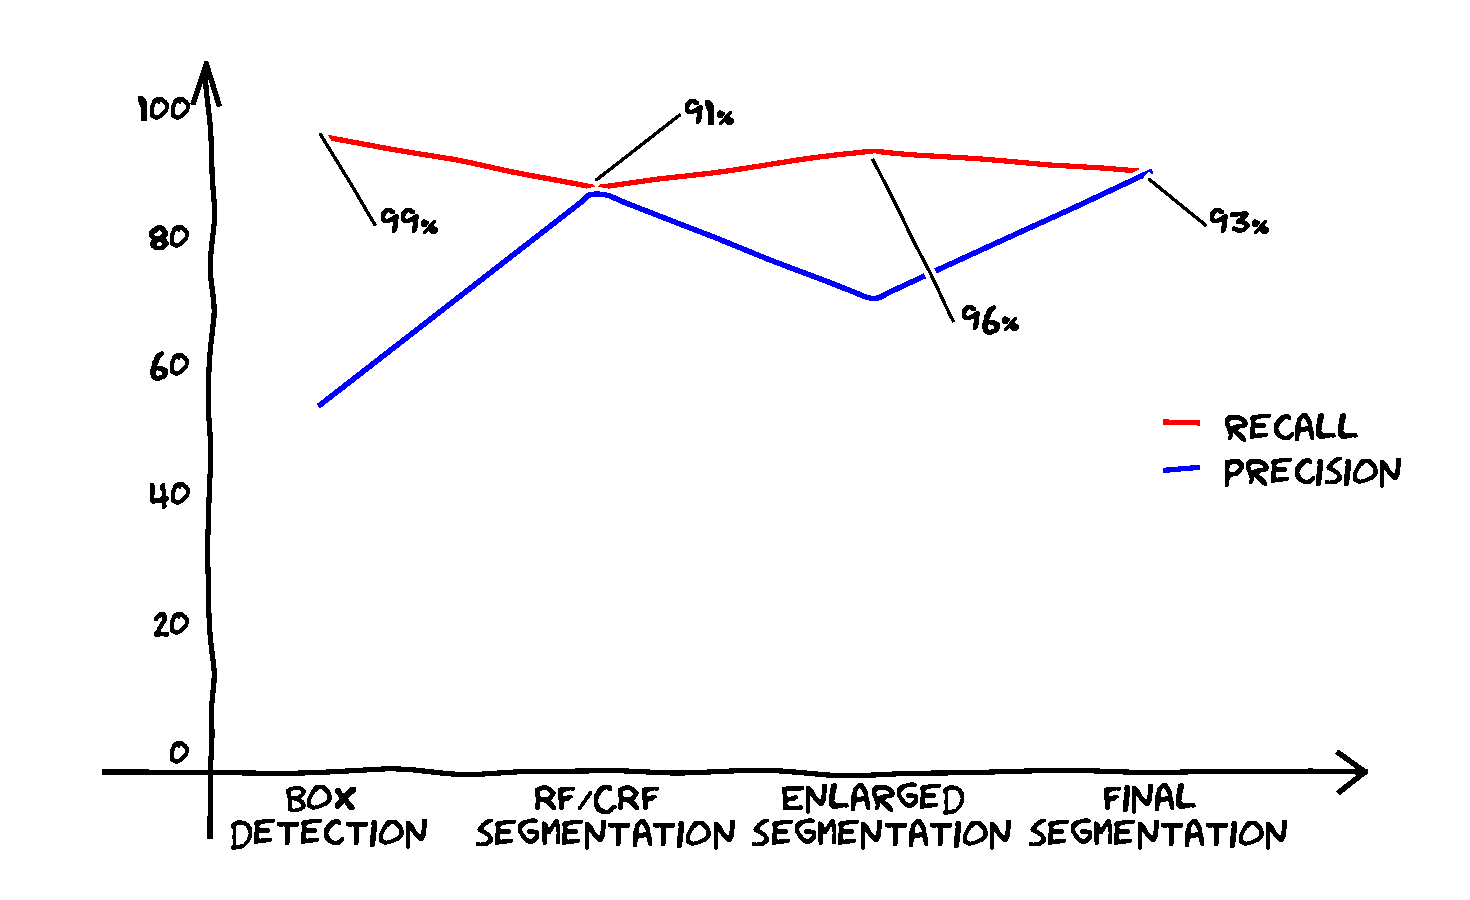
\includegraphics[height=0.8\textheight]{plot2.pdf}
\end{center}
\end{frame}

\begin{frame}{Box detection}

\vspace{0.025\textheight}

\centering


    

\begin{tikzpicture}[decoration=penciline]
    % Place nodes
    \node [block,text width=1.35cm,node distance = 2.45cm] (mser) {MSER};
    \node [block, right of=mser,text width=2.3cm,node distance = 2.55cm,] (size) {Size filtering};
    \node [block, right of=size, text width=2.5cm,node distance = 3.05cm,] (bag) {Bag-of-SIFT};
    \node [block, right of=bag,text width=1.6cm,node distance = 2.7cm,] (ransac) {RANSAC};
    \path [line]  (mser) -- (size);
 \path [line] (size) -- (bag);
\path [line] (bag) -- (ransac);

\end{tikzpicture}

\vspace{0.02\textheight}

\begin{minipage}{0.3\textwidth}
\centering
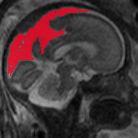
\includegraphics[width=0.45\textwidth]{img/mser/3.png}

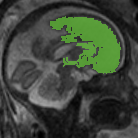
\includegraphics[width=0.45\textwidth]{img/mser/4.png}

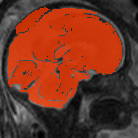
\includegraphics[width=0.45\textwidth]{img/mser/5.png}

MSER regions
\end{minipage}
\begin{minipage}{0.65\textwidth}
\centering
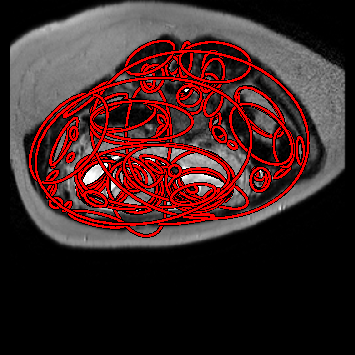
\includegraphics[width=0.5\textwidth,clip=true,trim=0 51 0 0]{30_all_mser.pdf}

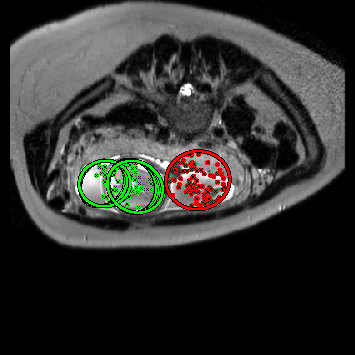
\includegraphics[width=0.5\textwidth,clip=true,trim=0 51 0 0]{30_selected_mser.pdf}

Filtering by size and Bag-of-Words
\end{minipage}
\end{frame}

\begin{frame}{Box detection}

\centering

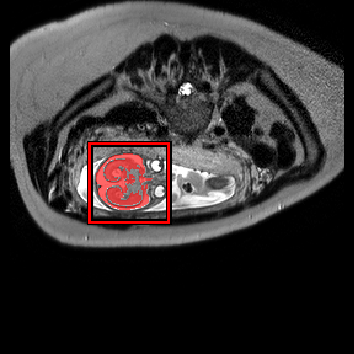
\includegraphics[width=0.65\textwidth,clip=true,trim=0 51 0 0]{maskZ.pdf}

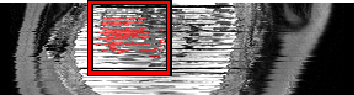
\includegraphics[width=0.65\textwidth]{maskY.pdf}

\end{frame}

\begin{frame}{Brain extraction}

\centering

Random Forest classifier

\vspace{0.01\textheight}

 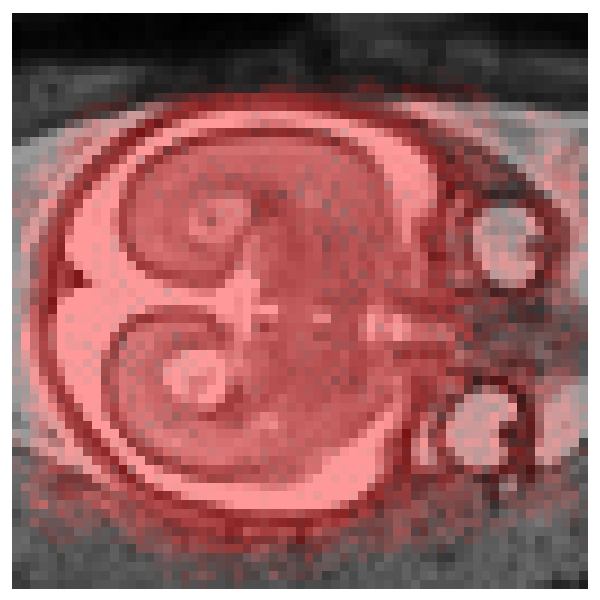
\includegraphics[width=0.3\textwidth]{3599_5_probaXY.png}
 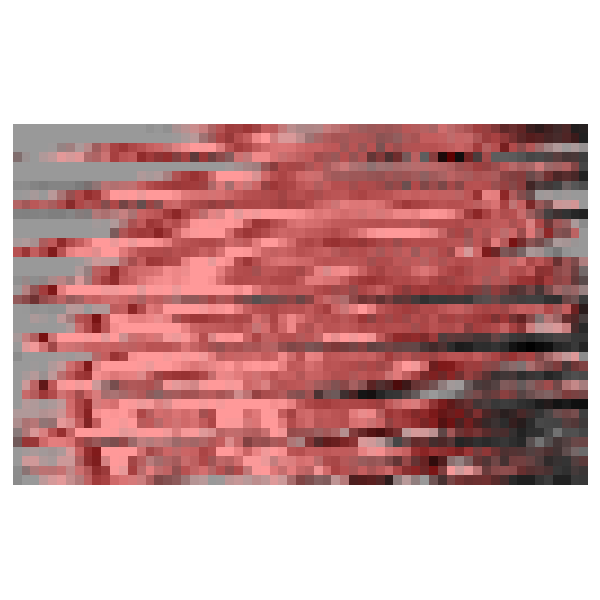
\includegraphics[width=0.3\textwidth]{3599_5_probaXZ.png}

 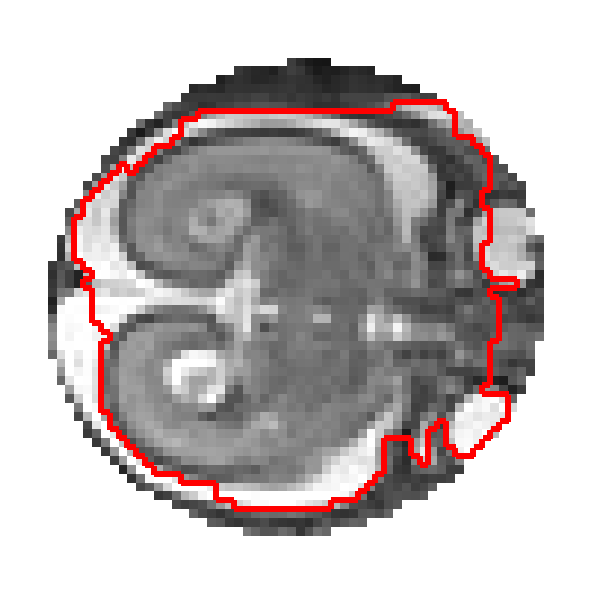
\includegraphics[width=0.3\textwidth, clip=true, trim=0 60 0 51]{3599_5_maskedXY.png}
 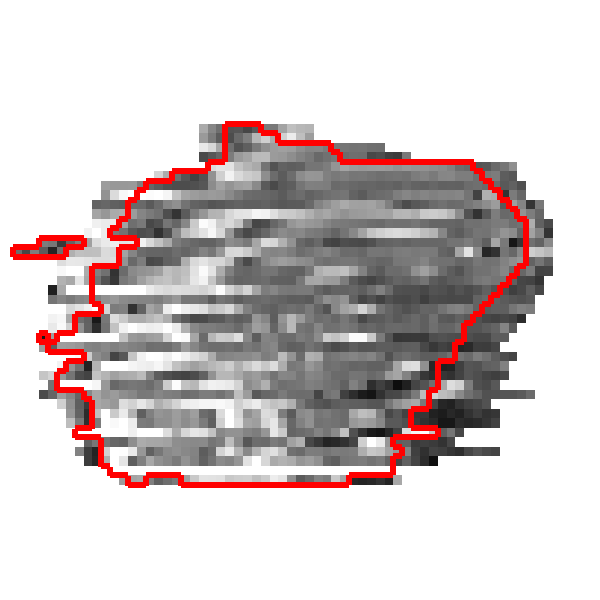
\includegraphics[width=0.3\textwidth, clip=true, trim=0 60 0 51]{3599_5_maskedXZ.png}

 and Conditional Random Field

\end{frame}

\begin{frame}{Motion correction}

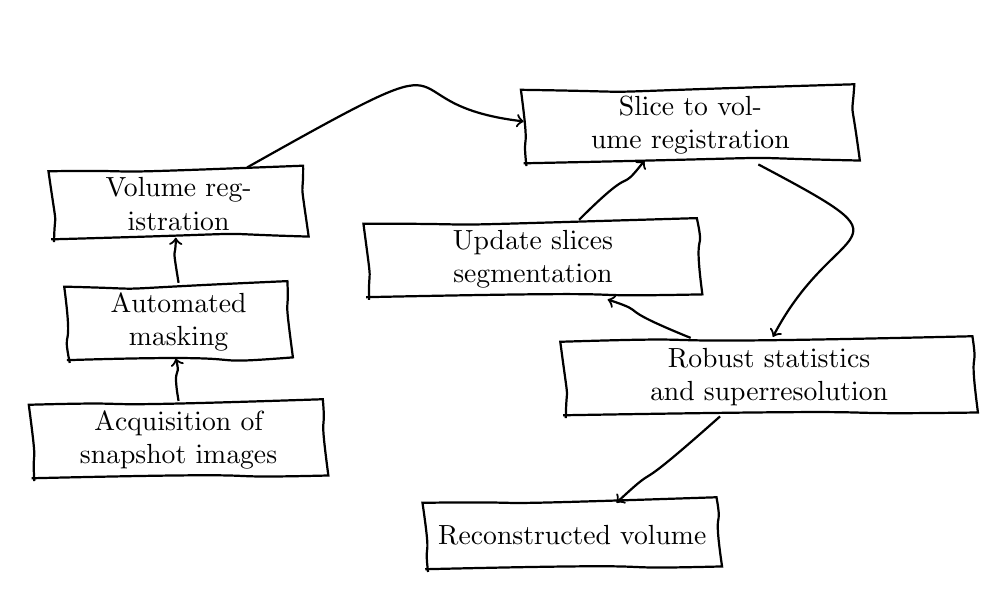
\begin{tikzpicture}[decoration=penciline]
    % Place nodes
    \node [block,text width=3.5cm] (acquisition) at (0,0)
    {Acquisition of snapshot images};
%above of=acquisition,
    \node [block, text width=2.6cm] (masking) at (0,1.5)
    {Automated masking};
%above of=masking,
    \node [block, text width=3cm] (volumeRegistration) at
    (0,3) {Volume registration};

%right of=volumeRegistration,
    \node [block, text width=4cm] (sliceRegistration) at
    (6.5,4) {Slice to
      volume registration};
%right of=masking,
    \node [block, text width=4cm] (update) at (4.5,2.3) {Update slices
    segmentation};
% %right of=update,
    \node [block, text width=5cm] (superresolution) at (7.5,0.8) {Robust
      statistics and superresolution};


%right of=acquisition,
    \node [block, text width=3.5cm,node distance = 6cm] (output) at (5,-1.2)
    {Reconstructed volume};

    \path [line]  (acquisition) -- (masking);
 \path [line] (masking) -- (volumeRegistration);
\draw [line] (volumeRegistration) to[out=28,in=180] (sliceRegistration);

\path [line] (sliceRegistration) to[out=-30,in=90] (superresolution);
\path [line] (superresolution) -- (update);
\path [line] (update) -- (sliceRegistration);

\path [line] (superresolution) -- (output);
\end{tikzpicture}

\end{frame}

\begin{frame}{Motion correction}

\centering

Conditional Random Field

\vspace{0.02\textheight}

 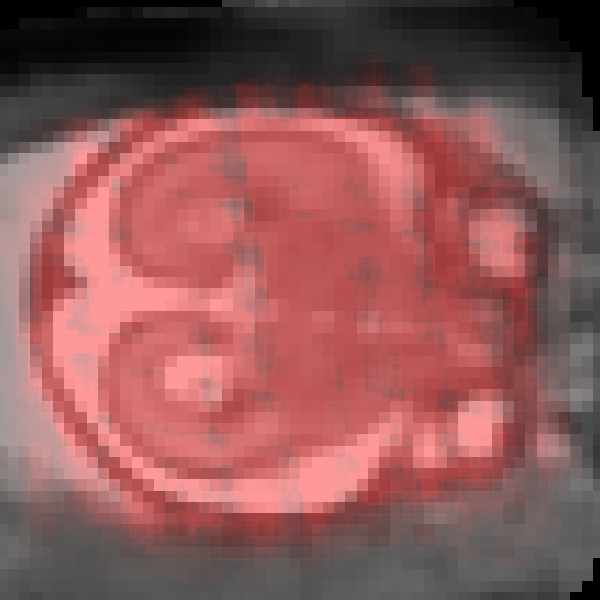
\includegraphics[width=0.3\textwidth]{3599_probabeforeCRFXY.png}
\hspace{0.01\textwidth}
 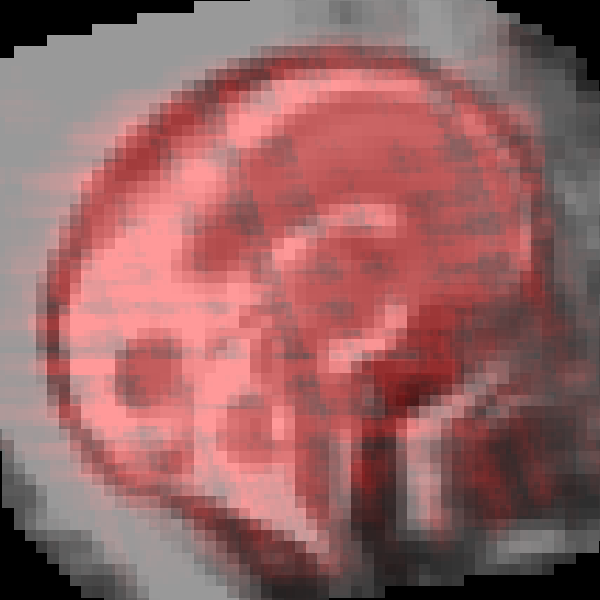
\includegraphics[width=0.3\textwidth]{3599_probabeforeCRFXZ.png}

 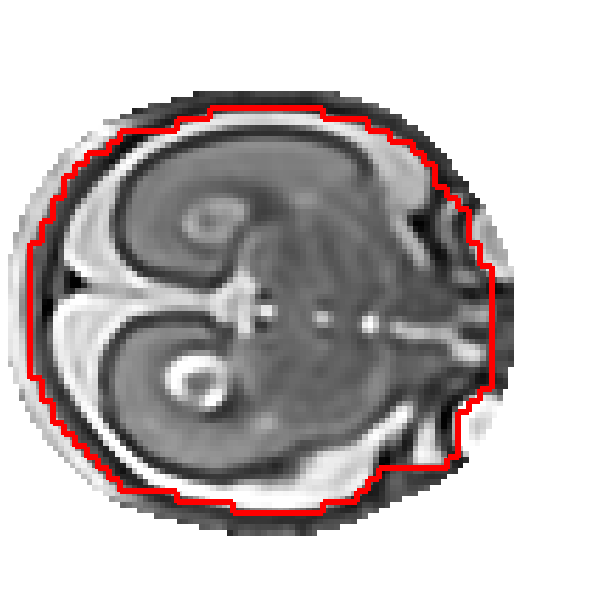
\includegraphics[width=0.3\textwidth, clip=true, trim=0 30 0 20]{3599_reconstructedXY.png}
\hspace{0.01\textwidth}
 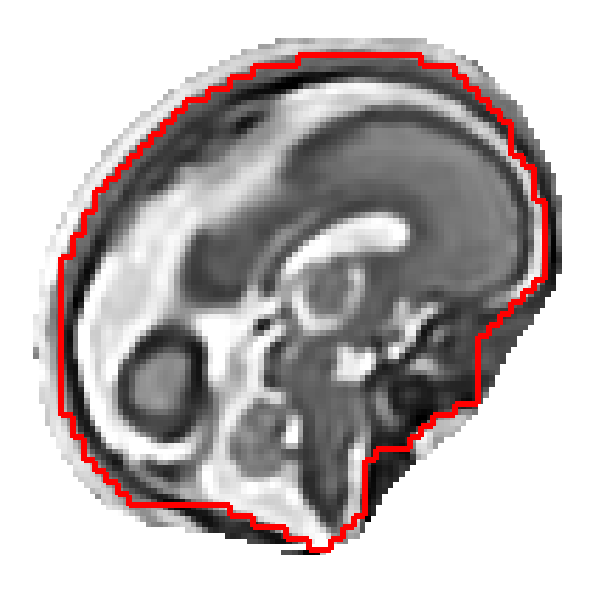
\includegraphics[width=0.3\textwidth, clip=true, trim=0 30 0 20]{3599_reconstructedXZ.png}

\end{frame}

\begin{frame}{Result}

\centering

 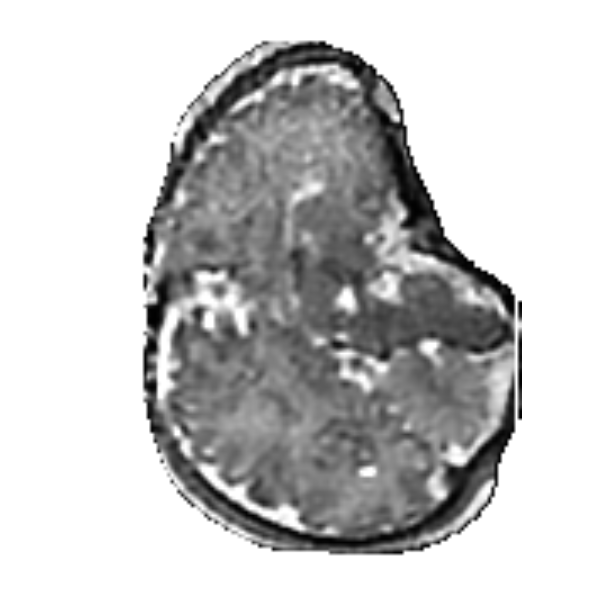
\includegraphics[clip=true, trim=90 0 45 0,angle=-90,width=0.3\textwidth]{white_2628_maskingXZ.png}
 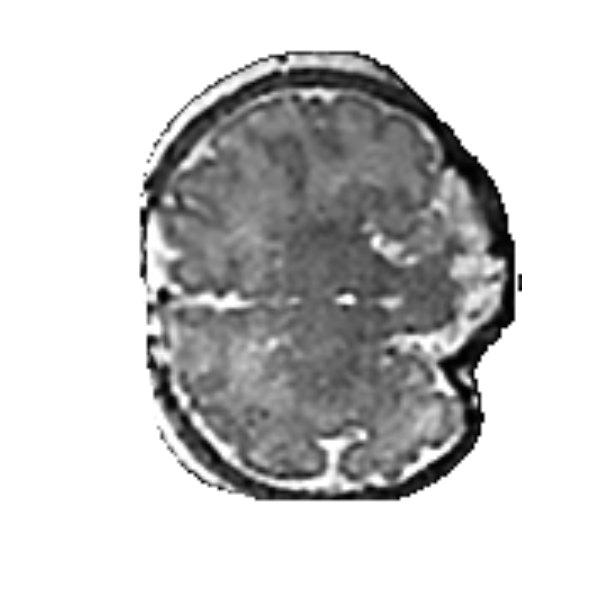
\includegraphics[clip=true, trim=90 0 45 0,angle=-90,width=0.3\textwidth]{white_2628_maskingXY.png}

 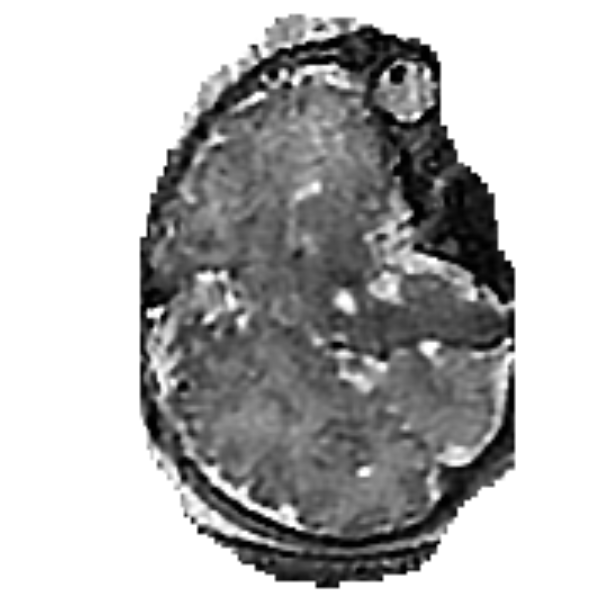
\includegraphics[clip=true, trim=35 0 25 0,angle=-90,width=0.3\textwidth]{white_2628_nomaskingXZ.png}
 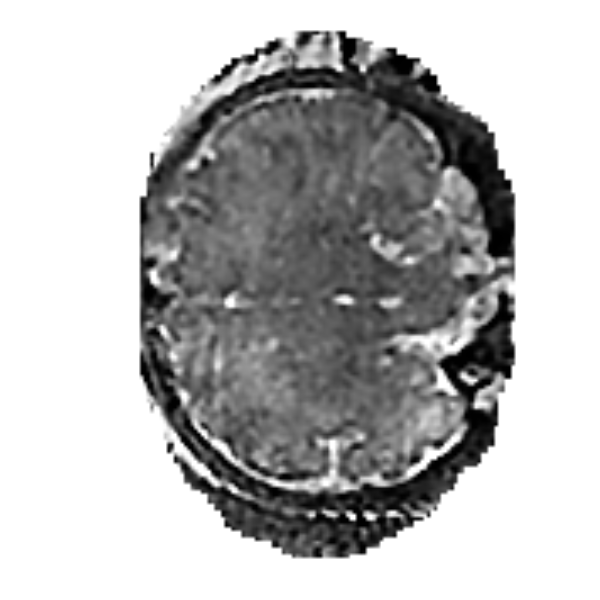
\includegraphics[clip=true, trim=35 0 25 0,angle=-90,width=0.3\textwidth]{white_2628_nomaskingXY.png}

Tighter mask, less artifacts\\
 and brain already extracted

\end{frame}

\begin{frame}{Acknowledgements}

\begin{itemize}

\item Collaborators:\\
Maria Murgasova,
Vanessa Kyriakopoulou, Christina
Malamateniou, Mary Rutherford, Bernhard
Kainz, Jo Hajnal \& Daniel Rueckert

\vspace{0.06\textheight}

\item XKCD for Matplotlib, Latex and Tikz:\\
\href{http://jakevdp.github.io/blog/2012/10/07/xkcd-style-plots-in-matplotlib/}{Jake
  Vanderplas},
\href{http://www.mail-archive.com/matplotlib-users@lists.sourceforge.net/msg25499.html}{Damon McDougall},
\href{https://github.com/JohannesBuchner/matplotlib-xkcdify}{Johannes Buchner},
\href{http://tex.stackexchange.com/questions/39296/simulating-hand-drawn-lines}{percusse}

\end{itemize}

\vspace{0.01\textheight}

\begin{center}
\large
\color{xkcd_color}
\href{http://www.doc.ic.ac.uk/~kpk09/}{www.doc.ic.ac.uk/\textasciitilde kpk09/}
\end{center}
\end{frame}

\end{document}
% ------ fin document ------
